\section{Понятие стека. Операции над стеком. Программная реализация стека на основе статического массива}
\subsection{Понятие стека}
Стек~--- абстрактный тип данных, представляющий собой список элементов, организованных по принципу
LIFO (англ. last in -- first out, «последним пришёл -- первым вышел>>). Стеки могут построены на основе других, более фундаментальных
структурах данных, например, можно реализовать стек как обертку над массивом с указателем или на основе списка. Проще говоря, стек представляет
собой абстрактный интерфейс доступа к данным, а не конкретную структуру данных.

Организация данных по принципу LIFO означает, что элементы могут добавляться и извлекаться только с вершины стека. При этом при добавлении
элемента, именно он становится новой вершиной стека, а при удалении, вершиной становится предыдущий элемент.

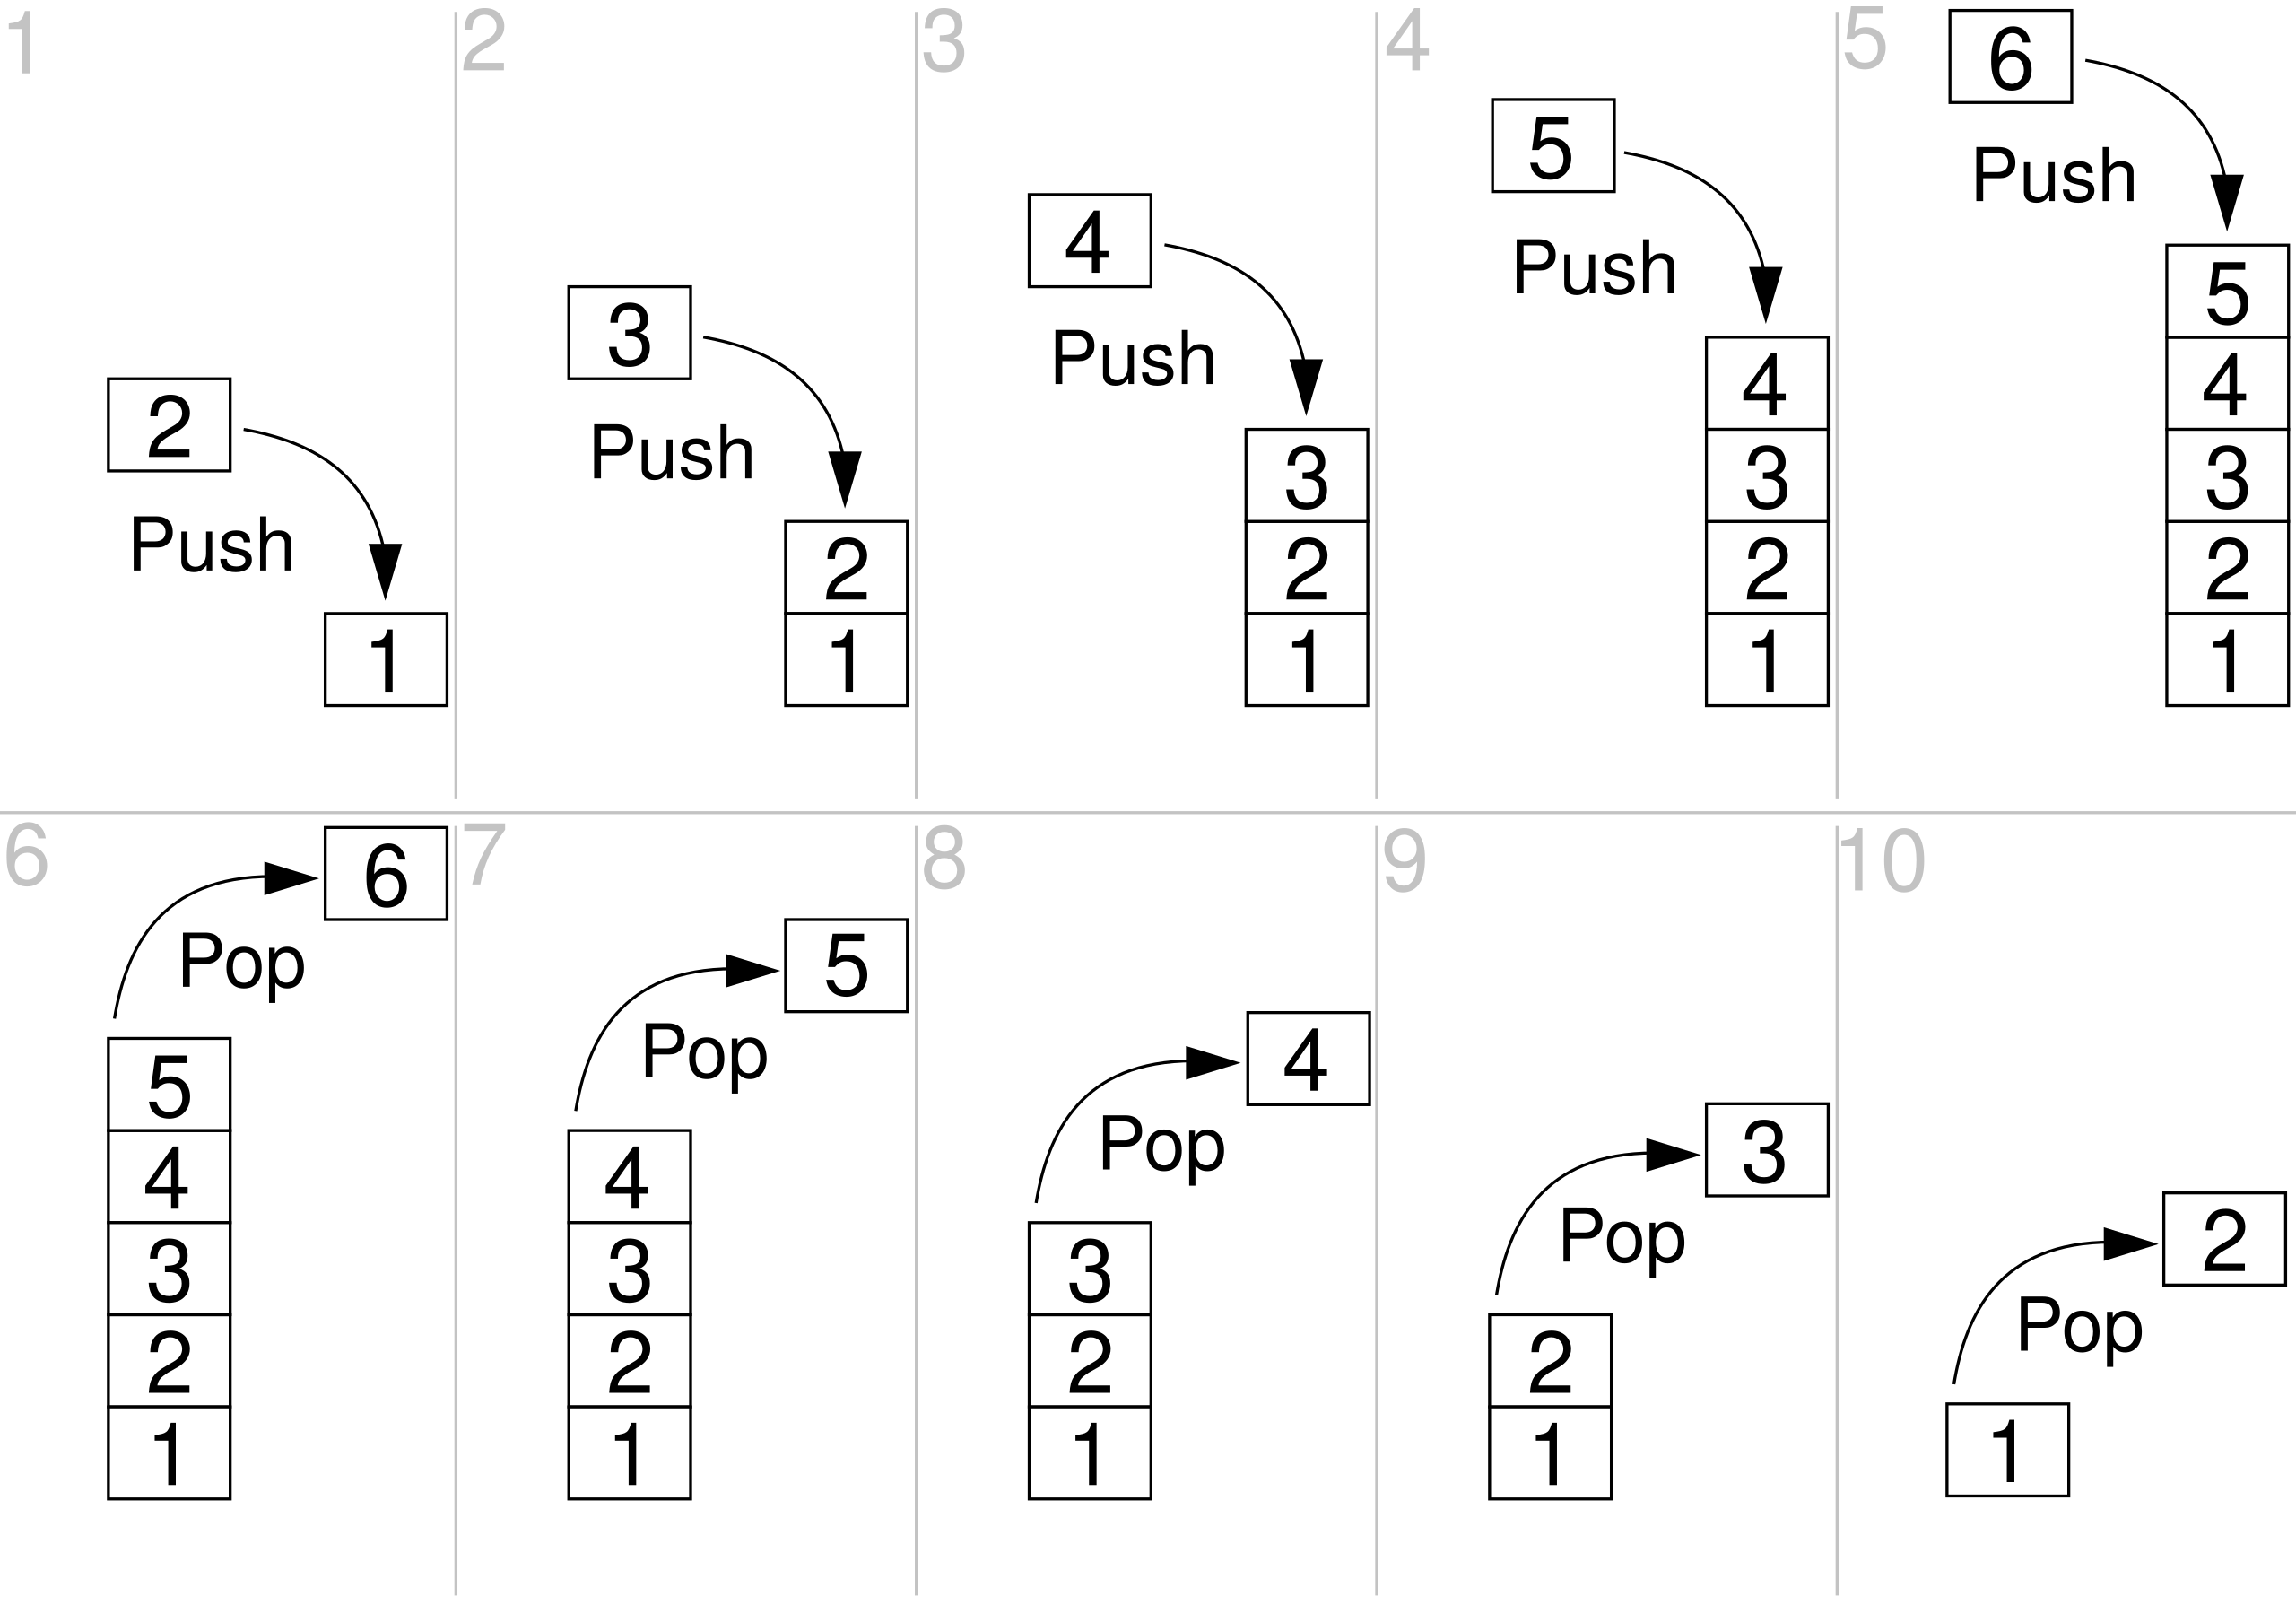
\includegraphics[width=0.9\textwidth]{resources/19-26/stack.png}

В стандартной библиотеке С++ присутствует реализация \cppref[стека]{cpp/container/stack}, объявленная в соответствующем
\cppref[заголовке]{cpp/header/stack}. Стоит отметить, что шаблон \mverb{std::stack<T>} не является
структурой данных сам по себе, а лишь предоставляет интерфейс стека поверх какой-либо другой структуры (по умолчанию, \cppref[\texttt{std::deque<T>}]{cpp/container/deque}).
Помимо этого, в качестве стека можно тривиально использовать динамический массив \cppref[\texttt{std::vector<T>}]{cpp/container/vector} с его
методами \mverb{push_back(T &&)}, \mverb{back()} и \mverb{pop_back()}.
\subsection{Операции над стеком}
Когда речь идет о стеке, подразумевается структура данных со следующими операциями:
\begin{enumerate}
    \item Добавить элемент в верхушку стека (\mverb{push()}).
    \item Удалить элемент из верхушки стека (\mverb{pop()}).
\end{enumerate}

Часто также требуется поддержка операции чтения вершины без ее удаления (\mverb{peek()}, также \mverb{top()}) и
проверки на пустоту (\mverb{empty()}).

\subsection{Пример реализации стека}
Приведем реализацию стека на основе статического массива фиксированной длины. Данная структура данных будет использовать шаблоны и \cppref[\texttt{assert(bool)}]{cpp/error/assert}
для проверок инвариантов.

\section{Понятие очереди. Операции над очередями. Кольцевая очередь. Деки.  Программная реализация очереди на основе статического массива}
\section{Использование очередей при реализации запросов ввода-вывода. Структура данных «список»}
\section{Программная реализация очереди на основе статического массива}
\section{Многократный поиск на основе использования статистических данных}
\section{Нечеткий поиск – поиск «подобной» подстроки. Бинарный поиск}
\section{Рекурсия: общий вид, свойства, проблемы. Стек вызова функций}
\section{Сортировки – общая классификация. Сортировки с помощью включения, выделения, обменов}
